\documentclass[tikz, border=10 mm]{standalone}
\usepackage[utf8]{vietnam}
\usepackage{tikz}
\usetikzlibrary{calc,decorations.pathmorphing}
\begin{document}
	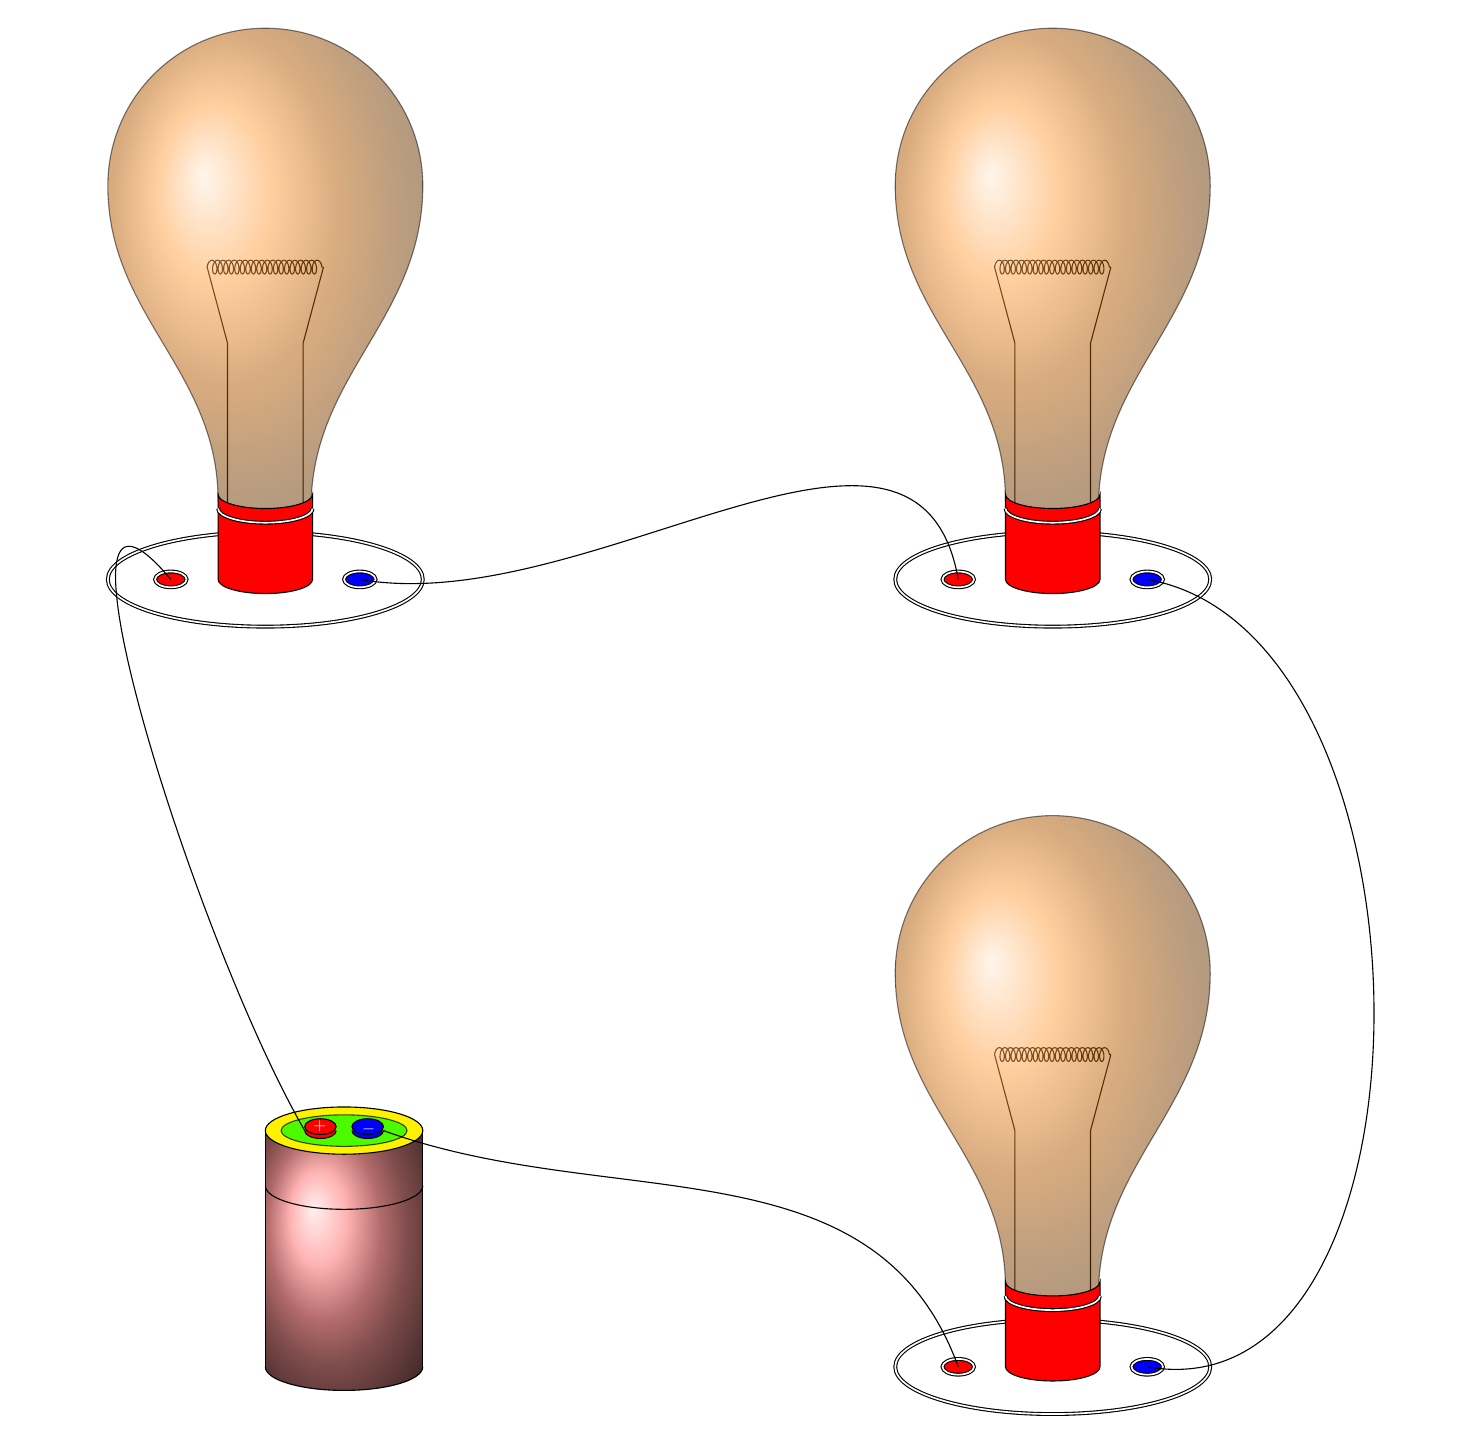
\begin{tikzpicture}
		%code đèn
		\def\den(#1,#2)(#3,#4){
			\begin{scope}[shift={(#1,#2)}]
				\def\a{2} \def\b{.6} \def\d{3}
				\draw[double] (0,0) ellipse ({\a} and {\b});
				\draw[double,fill=red] (-1.2,0)coordinate (#3) ellipse ({0.2} and {0.1});
				\draw[double,fill=blue] (1.2,0)coordinate (#4) ellipse ({0.2} and {0.1});
				\draw
				(-.24*\a,0)--++(90:\d)--++(105:1) coordinate (A)
				(.24*\a,0)--++(90:\d)--++(75:1) coordinate (B);
				\draw[decorate,decoration={coil,segment length=2pt}]
				(A)--(B);
				%\def\den{
					% (.29*\a,1.5*\b) to[out=90,in=-90]++(70:3.5)
					% to[out=90,in=0] (0,6);}
				%\draw \den; \draw[xscale=-1] \den;
				\draw[ball color=orange, opacity=0.5] (.29*\a,1.5*\b) to[out=90,in=-90] (2,5) to [out=90,in =0] (0,7) to[out=180,in=90] (-2,5) to[out=-90,in=90] (-0.6,1) arc (-180:0:{0.6} and {0.2});
				\draw[fill=red] (.3*\a,0) arc(0:-180:{.3*\a} and {.3*\b})--++
				(90:1.8*\b) arc(-180:0:{.3*\a} and {.3*\b})--cycle;
				\draw[double] (.3*\a,0) ++(90:1.5*\b) arc(0:-180:{.3*\a} and {.3*\b});
			\end{scope}
		}
		%code pin
		\def\pin(#1,#2)(#3,#4){
			\begin{scope}[shift={(#1,#2)}]
				\shade[ball color=red!40] (0,0) arc(180:360:1 and 0.3)--(2,3) arc(0:-180:1 and 0.3)--cycle;
				\draw (0,0)--(0,3)(2,0)--(2,3);
				\draw (0,0) arc(180:360:1 and 0.3);
				\draw (0,2.3) arc(180:360:1 and 0.3);
				\draw[fill=yellow] (0,3) arc(180:540:1 and 0.3);
				\draw[xshift=0.2cm,fill=green,opacity=0.7] (0,3) arc(180:540:0.8 and 0.2);
				\draw[shift={(0.5,0)},fill=red] (0,3)coordinate (#3) arc(180:360:0.2 and 0.1);
				\draw[shift={(1.1,0)},fill=blue] (0,3) arc(180:360:0.2 and 0.1)coordinate (#4);
				\draw[shift={(0.5,0.05)},fill=red] (0,3)node[scale=0.6,white,xshift=0.32cm]{$+$} arc(180:540:0.2 and 0.1);
				\draw[shift={(1.1,0.05)},fill=blue] (0,3)node[scale=0.6,white,shift={(0.35,-0.05)}]{$-$} arc(180:540:0.2 and 0.1);
			\end{scope}
		}
		\pin(0,0)(pinA,pinB)%vị trị và đặt tên các cực viên pin
		\den(10,0)(motA,motB)%vị trí và đặt tên các cực đèn thứ nhất
		\den(10,10)(haiA,haiB)
		\den(0,10)(baA,baB)
		\draw (pinA) to[out=120,in=130] (baA);
		\draw (baB) to[out=-10,in=100] (haiA);
		\draw (haiB) to[out=-10,in=-10] (motB);
		\draw (motA) to[out=110,in=-20] (pinB);
	\end{tikzpicture}
\end{document}